% THIS IS SIGPROC-SP.TEX - VERSION 3.1
% WORKS WITH V3.2SP OF ACM_PROC_ARTICLE-SP.CLS
% APRIL 2009
%
% It is an example file showing how to use the 'acm_proc_article-sp.cls' V3.2SP
% LaTeX2e document class file for Conference Proceedings submissions.

\documentclass{acm_proc_article-sp}

\begin{document}

\title{uF!t: A Framework for Monitoring Exercises}

% \subtitle{[Extended Abstract]
% \titlenote{A full version of this paper is available as
% \textit{Author's Guide to Preparing ACM SIG Proceedings Using
% \LaTeX$2_\epsilon$\ and BibTeX} at
% \texttt{www.acm.org/eaddress.htm}}}

%
% You need the command \numberofauthors to handle the 'placement
% and alignment' of the authors beneath the title.
%
% For aesthetic reasons, we recommend 'three authors at a time'
% i.e. three 'name/affiliation blocks' be placed beneath the title.
%
% NOTE: You are NOT restricted in how many 'rows' of
% "name/affiliations" may appear. We just ask that you restrict
% the number of 'columns' to three.
%
% Because of the available 'opening page real-estate'
% we ask you to refrain from putting more than six authors
% (two rows with three columns) beneath the article title.
% More than six makes the first-page appear very cluttered indeed.
%
% Use the \alignauthor commands to handle the names
% and affiliations for an 'aesthetic maximum' of six authors.
% Add names, affiliations, addresses for
% the seventh etc. author(s) as the argument for the
% \additionalauthors command.
% These 'additional authors' will be output/set for you
% without further effort on your part as the last section in
% the body of your article BEFORE References or any Appendices.

\numberofauthors{2}

%\author{
% You can go ahead and credit any number of authors here,
% e.g. one 'row of three' or two rows (consisting of one row of three
% and a second row of one, two or three).
%
% The command \alignauthor (no curly braces needed) should
% precede each author name, affiliation/snail-mail address and
% e-mail address. Additionally, tag each line of
% affiliation/address with \affaddr, and tag the
% e-mail address with \email.
%
% 1st. author
% \alignauthor
% Ben Trovato\titlenote{Dr.~Trovato insisted his name be first.}\\
%        \affaddr{Institute for Clarity in Documentation}\\
%        \affaddr{1932 Wallamaloo Lane}\\
%        \affaddr{Wallamaloo, New Zealand}\\
%        \email{trovato@corporation.com}
% % 2nd. author
% \alignauth`or
% G.K.M. Tobin\titlenote{The secretary disavows
% any knowledge of this author's actions.}\\
%        \affaddr{Institute for Clarity in Documentation}\\
%        \affaddr{P.O. Box 1212}\\
%        \affaddr{Dublin, Ohio 43017-6221}\\
%        \email{webmaster@marysville-ohio.com}
% }

\author{
\alignauthor
Brandon Snuggs\\
       \affaddr{Swarthmore College}\\
       \affaddr{500 College Avenue}\\
       \affaddr{Swarthmore, Pennslyvania}\\
       \email{bsnuggs1@swarthmore.edu}
% 2nd. author
\alignauthor
Steven Hwang\\
       \affaddr{Swarthmore College}\\
       \affaddr{500 College Avenue}\\
       \affaddr{Swarthmore, Pennslyvania}\\
       \email{shwang1@swarthmore.edu}
}

\maketitle
\begin{abstract}
Common reasons for the low motivation to exercise include
the absence of an exercise partner and the large time invest-
ment required in traveling to the gym. Some responses to this
issue have divulged possible solutions: joining an exercise
support groups or focusing on exercises that can be done with-
out gym equipment. While both suggestions are practical, 
studies show support groups are notable in that they have 
been known to be effective at keeping individuals adhere to a
regular exercise routine. Furthermore, the modern evolution of
social networking sites has allowed for support groups to form
online.

It should be noted that there are a multide of engaging
exercises that can be done with minimal gym equipment 
(i.e. pushups, situps, yoga); however, it is often a hassle to
mentally keep track of all these exercises. We present uF!T, as
a framework that leverages the benefits of exercise support
groups and provides tools to monitor and count exercises done
inside and outside the gym. uF!T attempts to take advantage 
of static position measurement accuracy in an accelerometer
and the smoothness of gyrometer measurements in a complementary
filter to reduce noisy measurements. Our evaluation of uF!t
includes experiments on proper sensor placement and will 
include tests on classification accuracy.
\end{abstract}

\section{Introduction}
Currently, America's healthcare costs have been rising more 
and more each year. One of the most influencing factors in this
phenomenal increase is due to obesity. In 2008, obesity health-
care costs account for at least 10 of total medical expenditures.
This amounts to 147 million dollars a year. While exercise is a
the main solution to help reducing obesity, the increase in 
fast-paced lifestyles and lack of motivation has caused going to
the gym to be cut from most schedules. Many mobile application 
developers have sought to provide creative solutions that comple-
ment a packed schedule and low interest in exercising. Mobile 
devices such as smartphones, ipods, and chips built-in shoes now
are equipped with considerable computational power and are very
portable. Furthermore, work with wireless sensor networks has 
been done to classify exercises done in the gym []. Some notable
examples of mobile devices are as follows: Nike fit (an ipod 
application that is available on most ipod devices) is available
on many Ipod devices as an application that encourages users to
run by logging the distance run, calories burned and time of an
individual�s runs. Another application is Zombierun which has 
sought to encourage individuals to exercise by introduce a gaming
aspect to the routine as well as the ability to share results via
social media. The Zombierun application has shown to be successful
by popular account (stats???) [] and has therefore involved 
encouraged many people to exercise more. The Zombierun application
however, is limited to running. We present uF!t as a wireless
sensor network that would extend tracking exercise to gym and
incorporate the gaming and social media aspects to motivate 
individuals who are inclined to exercise at the gym.

\subsection{Why don't people exercise?}
Dunno. You tell me.

\section{SYSTEM ARCHITECTURE}
Our system will consist of the following components: Workout 
classifier, exercise counter, wireless data transfer protocol 
and Social Media application.

\subsection{Workout classifier}
uF!T will interpret accelerometer and gryoscope data in order
to determine what exercise is being performed. Our current 
classifier will distinguish exercises according to sensor 
measurement values along the x, y and z axes. Sensors measure-
ments would include rotational velocity around each axis and 
acceleration along each axis and be stored in a 6-tuple. The
k-means classification algorithm would be used to group sets 
of sensor measurements into clusters where we assume each 
cluster would represent an exercise. (Describe store the 
exercise measurement values in a file for describing the 
exercises....).

Therefore, successive measurements that obtain values that are
similar in value to a cluster would be grouped with it. 
Practically, the classifier would consider a fixed number 
(100 samples) of sensor measurements at a time.

The following describes the k-means algorithm:

\begin{enumerate}
\item Place K points into the space represented by the objects that are being clustered. These points represent initial group centroids.
\item Assign each object to the group that has the closest centroid.
\item When all objects have been assigned, recalculate the positions of the K centroids.
\item Repeat Steps 2 and 3 until the centroids no longer move. This produces a separation of the objects into groups from which the metric to be minimized can be calculated.
\end{enumerate}

After clusters are determined, we would classify incoming data
according to which cluster center they most resemble. We note
that we have not classified the characteristics of many exercises
besides a situp. Furthermore, it is possible to have an individual
do an exercise that is currently not defined. In this case, this
exercise would be classified as an unknown exercise and still be
tracked and counted. For practical purposes it is likely for some
exercises to not be defined given the limited space on the mote 
that is available to store exercise classification information.
Nevertheless, the user would be given the option of specifying a
name for this exercise so that it could be tracked in the future.

\subsection{Exercise Counter}
After an exercise has been classified we would begin counting 
features of the exercises in order to keep track of the number 
of repetitions that have been completed. We note that many exer-cises
are characterized by a repeated movement and can therefore be 
partitioned based off peaks that may occur during the exercise.
(other ways of partitioning ?.....).  Therefore, by counting the 
number of peaks that occur in during the exercise, would be able
to achieve an accurate account of the number of repetitions that 
were completed.

\subsection{Peak detection}
In order to recognize a peak in the measurement data, we would
set threshold values that would represent the minimum value to
be considered a peak and the maximum value to be considered a 
pause or rest between repetitions. Each peak in the measurement
readings would consist of data points that are above the peak 
threshold value. It is common to have multiple data points 
classify to be a peak value. The number of successive peak values
indicate confidence that a peak is correctly observed. Typically,
higher frequencies in a given would indicate a stronger confidence
that a peak is indeed there while lower frequencies (one or two 
peak detections) might indicate some noise. In order to make our 
system more robust to misclassification due to noise we propose 
the following conditions:

\begin{enumerate}
\item In order to be classified as a peak there must be at least 3 consecutive peak classifications. Otherwise, the classification is assumed to be from noise.
\item If a peak is classified recently another peak classification would be counted toward the recent peak instead of classifying a new peak.
\end{enumerate}

Furthermore, threshold values are initially chosen by hand. 
In order to account for the potential to have different forms of 
data for individuals, these threshold values will be user-specific.
We hope to gain this information by dynamically updating these 
threshold values and store these in a user profile on the social
media application.

\subsection{Wireless Protocol}
The motes will communicate with a base station based on a passive
architecture. Passive communication architecture has shown to 
reduce the usage of the motes radio for needless transmissions.
According to this architecture, a base station will constantly be
transmitting queries for information. Once a mote is within range
of a base station, the mote will attempt to establish stable 
connection and transmit the user�s exercise information.

The wireless protocol of this framework would also implement 
synchronous communication that would reduce the amount of time 
needed to listen for a response [123123].

Both features of the protocol are will increase the lifespan of
the mote�s battery. In order to reduce extraneous use of radio given
that the use of radio has been known to be a component that would
drain a mote�s battery the most rapidly [].

\subsection{Social Media Application}
Our framework plans to have a base station connect to a server for
storage of user profiles. Users would be able to login into a Facebook
application in order to view and share their exercise history with 
friends. A primary feature of the Facebook application would be the 
game component of the application. Users would rewarded for completing
exercise goals and in turn use their rewards to their advantage in an
online game. The game would involve a system where cumulative progress
is visible (i.e. building a fortress with upgraded turrets to defend 
against barbarian hordes). Furthermore, the Facebook application would
also serve to store user-specific information that would allow for 
dynamic exercise classification. Each user would have associated 
threshold values for each exercise they regularly complete. It is 
possible for these threshold values to be updated regularly (i.e. if
the user improves their form when engaging in exercises or if default
threshold values are too high or too low). Therefore, each time the base
station communicates with the mote and receives feedback on improving the
threshold values, the Facebook application would store these new threshold
values. (What about updating the threshold values in the mote????)

\begin{figure}
\centering
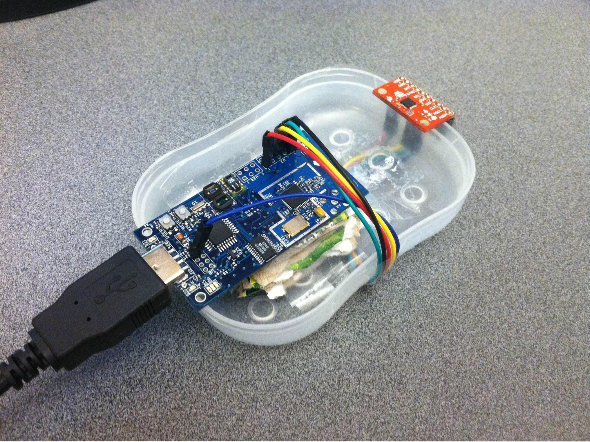
\includegraphics[width=2.0in,width=2in]{./figs/tmotesky.png}
\caption{The current casing for our uF!t device.}
\end{figure}

\section{Hardware and Software}
We decided to use the Tmote Sky for the basis of our project. The Tmote 
Sky can be powered by two AA batteries, however in our current 
implementation of uF!t, it is still wired, thus not requiring the use
of batteries.  Besides the electrical components, we have encased our
device using a lightweight plastic container (similar to a soap bar case).
The housing for our device helps the sensor sit in a stablize position.
The data is already noisy, so it is important that the sensors are not
given more opportunities to be mutated by noises induced by the sensor
rocking carelessly.


\subsection{Hardware: mpu6050}
We have connected the 3-axis Gyro/Accelerometer mpu6050.  The gyroscope
has sensitivity up to \(131 LSB/^\circ/s\), which can be easily
modified with Contiki functions that we have created. The mpu6050 sensor
also contained a temperature gauge; for the time being, we did not 
incorporate the temperature gauge into our project, but we believe it may
have later uses (for more info please look at future works).

\subsection{Software: Contiki 2.6}
Unlike a standard out-of-the-box Tmote Sky, we use Contiki 2.6, instead of
using TinyOs.  We chose to make this decision since our team was much
more familiar with C, which made it much easy for us to quickly
understand native functions in Contiki 2.6.  Additionally, this allowed
us to focus on understanding how to integrate the accelerometer and
gyroscope's functionality into Contiki.
	 	
\section{Implementation}
To ensure that we could track a user's body while doing a situp,
this required more work than just using the accelerometer and 
gyroscope raw data to do localization.  As such, we ran through
some equations that either used the accelerometer or the gyroscope.
However, after some strong analysis, in the end it required that 
we use both measurements in order to calculate the angle of user's
body.  The mpu6050 sensor that we used consisted of a 6-axis 
accelerometer and gyroscope.

\subsection{Accelerometer}
In order to track simple movements like a push-up or sit-up,
it was easy to determine by focusing on variation in the 
accelerometer's z (for the push-up) and the accelerometer's
y (for a pull-up).  However, in order to calculate the angle
of the user'ss body in respect to our sensor, it required some
trigonometry.

\begin{equation}angle_{accel_x} = \arctan(accel_x,accel_z) + \pi\end{equation}

Using the equation above allows us to calculate the tilt angle 
for the accelerometer.  Remember that arctan, known as atan2
in contiki, outputs between the range of \(-\pi\) and \(\pi\), so you
must add \(\pi\) to the results of arctan to have the range convert-
ed to 0 to 2\(\pi\).  Having no initial knowledge in the usage
of accelerometers or gyroscopes, we believed that the accelero-
meter would have served its purpose for calculating the wearer's
body angle during a situp.  However, if we look at figure 2
we can see that our initial assumption was clearly untrue.  The
accelerometer is great at calculating angles for stationary 
positions, but it is terrible at tracking the rapid movements 
experienced during a situp.  In figure 2, the data that 
we received was extremely noisy, so we were able to poorly track
the user's angle while doing a situp.  This lead us to try some
experiments with the gyroscope.

\begin{figure}
\centering
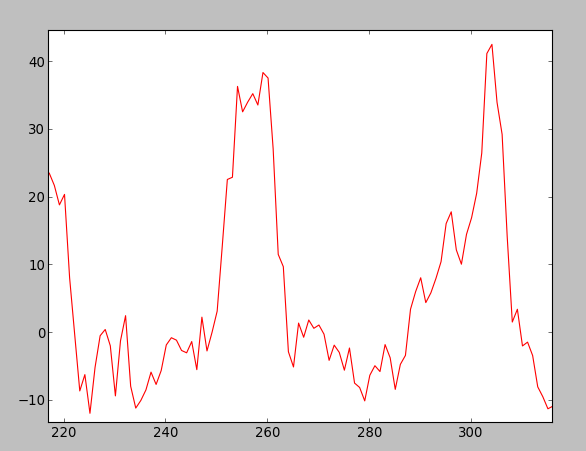
\includegraphics[width=3.0in,width=3in]{./figs/accel_test.png}
\caption{The results of the accelerometer, notice that
the data is extremely noisy.}
\end{figure}

\subsection{Gyroscope}
The gyroscope is able to calculate angular velocity in degrees 
per second, which lead us to think that the gyroscope would
provide more promising results.  For the gyroscope, we used 
this simple equation to calculate the angle.

\begin{equation}angle_{gyro_x} = angle_{gyro_x} + gyro_x*dt\end{equation}

Gyro is the degrees per second (\(^\circ/s\)) recorded from the
gyroscope, while delta t is the sample period calculated from 
the samplespeed.  In our trials, we used a sampling speed of 
20hz.  You can calculate the sample period from the sampling 
rate by using the following equation:

\begin{displaymath}T = 1/f\end{displaymath}

So for our trials, the sample period was .05.  Multiplying 
the gyro by sample period, it gives us the angle calculated 
within one cycle, which can be accumulated in our total angle.  
Successfully being able to calculate the angle using the gyro, 
we were certain that our results was going to be great.  Looking
at figure 3, however, the gyroscope's measurments are 
constantly increasing by a fixed amount as time goes on, this
is called \textit{drift}.  From our gryoscope analysis it seems that the
gyro not only experiences horrible drift (about \(5^\circ/s\)),
but it also is not centered properly.  When the gyroscope is
placed in a stationary position, it is expected to return a 
measurment of about 0 degrees per second.  In our studies, our
gyroscope actually returns about \(34^\circ/s\) when it is not
in motion.

\begin{figure}
\centering
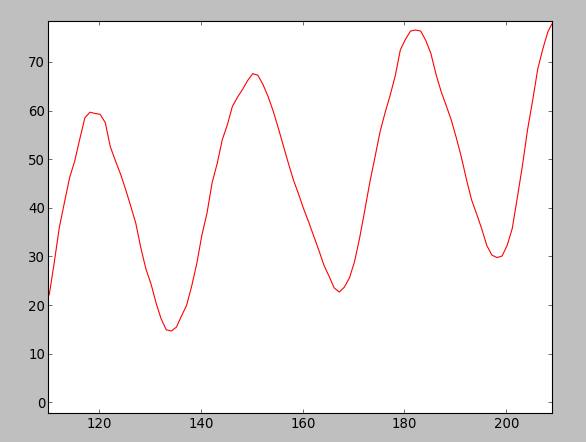
\includegraphics[width=3.0in,width=3in]{./figs/gyro_test.png}
\caption{The results of the accelerometer, notice that
the data is extremely noisy.}
\end{figure}


\subsection{Complimentary Filter}
From our analysis, we can see that both accelerometers and 
gyroscopes have their own pros and cons.  The accelerometer 
is really good at detecting static positions, however whenever
it is moving very quickly, it returns very noisy data.  In 
contrast, the gyroscope is really good at detecting rapid 
movements, however its data drifts over time, making it 
increasingly inaccurate the longer you monitor the gyroscope.
This lead us to using the complimentary filter.

\begin{equation}angle_x = (a)*(angle_x+gyro_x*dt)+(1-a)*(angle_{accel_x})\end{equation}

With the knowledge that we cannot rely on the gyroscope for 
long periods of time, it is important to calculate a good time
constant.  The time constant helps determine the coefficients 
used in the filter.

\begin{equation}\tau = \frac{a*dt}{1-a}\end{equation}

The time constant may vary from user to user depending on
the reliability of the gyroscope's data and the sample
rate.  The time constant defines the boundary between
trusting the gyroscope and trusting the accelerometer.
In our time constant, we used a time constant of \textit{.5
seconds}.  This means that for any measurement that is
lower than half a second, the algorithm will take the
gyroscope's measurements into consideration.  However,
for any measurements that take longer than half a second,
the accelerometer will have more weight, allowing it to
take precedence over the gyroscope.  Remembering that
the gyroscope drifts over time, it is better to trust
the accelerometer when the given time period is taking
too long.


\section{Evaluations}
In order to estimate how well our uF!t system is working, it
will require the evaluation of two things: Peak Detection
and Proper Sensor Placement.  Peak Detection allows us to
determine whether the user has successfully completed a situp
or not.  This algorithm is important in being able to correctly
detect a situp.  Without good recognition of a simple situp,
we would be unable to trust our system, which means that we
would not able to further implement new exercises on our system.
Proper Sensor Placement is important for making sure that
the data we record is consistent.  By placing uFit in neg-
lible areas, the data may suffer from additional unwanted 
noise, which would make it more difficult to detect good
exercises.

\subsection{Peak Detection}
There are two important terms that we use for our Peak
Detection algorithm: \textit{peaks} and \textit{rests}.
Peaks are moments where the user has effectively 

\subsection{Proper Sensor Placement}
For testing proper sensor placement, we proposed several
areas where the sensor could be placed on a user's body.
As stated earlier, it is important to choose a good loca-
tion for the system since it may affect the overall qual-
ity of the data.  Additionally, we must consider whether
or not if the placement of the sensor is comfortable for
the user.  In our prelimenary tests, it seems that it was
acceptable to place the device on the following three
places: \textit{the arm, center of chest, and the side 
of the chest.} We assumed that the center of the chest
would provide us with the most accurate data, since it
is centered at the body and it should not affect any of
the data since the chest area is generally an even area
for people of most sizes.

\begin{figure}
\centering
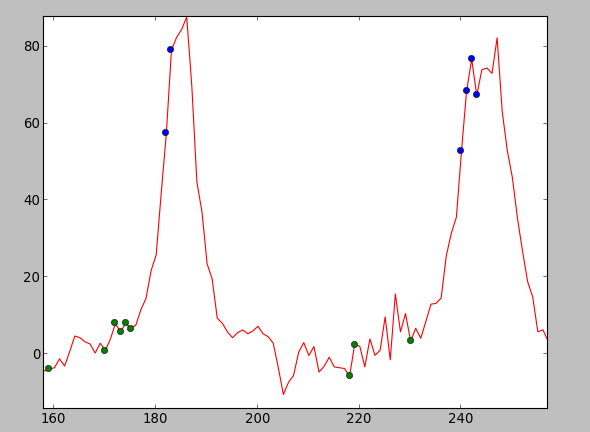
\includegraphics[width=3.0in,width=3in]{./figs/chestTestcenter.png}
\caption{The results of the complimentary filter with sensor placed
on the center of the chest.}
\end{figure}

\begin{figure}
\centering
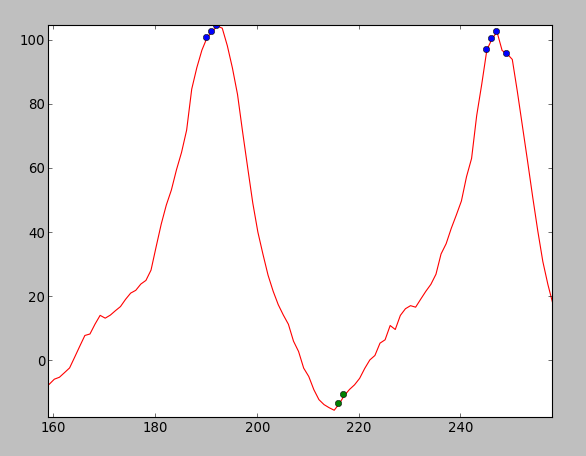
\includegraphics[width=3.0in,width=3in]{./figs/chestTestside.png}
\caption{The results of the complimentary filter with sensor placed
on the side of the chest.}
\end{figure}

Looking at the graphs depicted in Figures 6,7,8, we can see that
our initial assumption was actually incorrect.  It seems
that the sensor obtained the best results when it was
placed on the side of the chest.  Of course, we expected
that the arm would not be the best place since depending
on the user, they may either do a situp with their arms
placed on the side of their body, or they may do it with
their arms crossed across their chest.

These results were nice for our initial attempts, however,
we believe that it lacks the diversity of different sized
bodies for the test results.  We believe that if we can
get more people for our analysis, we can see if the positions
that we have provided are universally good for different
sized people.  So far our preliminary results have been
tested on average-sized males, which currently is a limited
scope of view considering that we wish this device to be
used by many people.

\begin{figure}
\centering
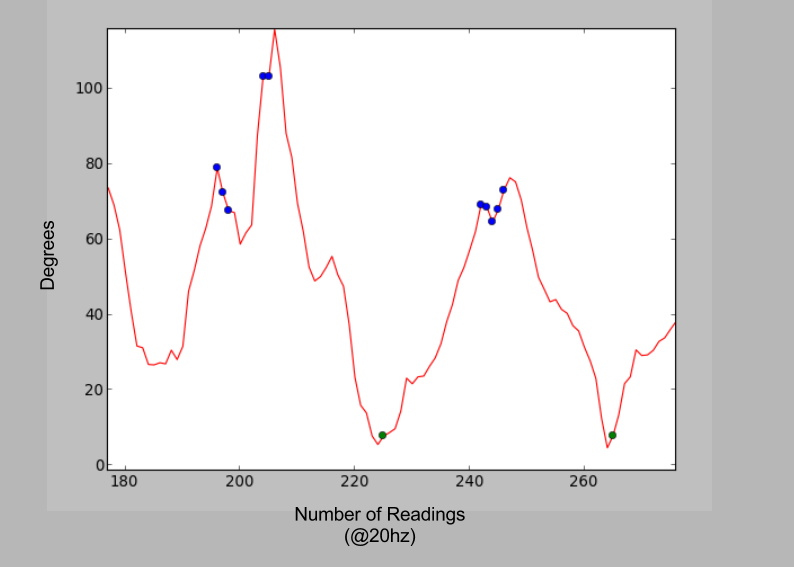
\includegraphics[width=3.0in,width=3in]{./figs/armTest.png}
\caption{The results of the complimentary filter with sensor placed
on the arm.}
\end{figure}

\section{Related Works}
In [], they rely on the raw measurements received from using
only 3-axis accelerometers.  However, unlike our design, they
use multiple accelerometers.  This allows their system to have
more versatility than the amount of exercises that we are
attempting to track.

\section{Future Works}
We note that we note that k-means is a na�ve solution that
is heavily dependent on the initial placement of the cluster
centers as terrible initial placements could introduce 
inaccuracies that are not completely eliminated by moving the
center. We look to implement a more advanced dynamic version 
of k-means that is touted to be more accurate "K-Harmonic Means"
[].

For dynamic peak detection would implement "general" peak 
detection that would search for inflection points in the data

We also take into account the fact that threshold values could be driven to values too low that noise would cause mis-classification.

\section{Conclusions}
This paragraph will end the body of this sample document.
Remember that you might still have Acknowledgments or
Appendices; brief samples of these
follow.  There is still the Bibliography to deal with; and
we will make a disclaimer about that here: with the exception
of the reference to the \LaTeX\ book, the citations in
this paper are to articles which have nothing to
do with the present subject and are used as
examples only.
%\end{document}  % This is where a 'short' article might terminate

%ACKNOWLEDGMENTS are optional
\section{Acknowledgments}
This section is optional; it is a location for you
to acknowledge grants, funding, editing assistance and
what have you.  In the present case, for example, the
authors would like to thank Gerald Murray of ACM for
his help in codifying this \textit{Author's Guide}
and the \textbf{.cls} and \textbf{.tex} files that it describes.

%
% The following two commands are all you need in the
% initial runs of your .tex file to
% produce the bibliography for the citations in your paper.
\bibliographystyle{abbrv}
\bibliography{final_report}  % sigproc.bib is the name of the Bibliography in this case
% You must have a proper ".bib" file
%  and remember to run:
% latex bibtex latex latex
% to resolve all references
%
% ACM needs 'a single self-contained file'!
%
%APPENDICES are optional
%\balancecolumns
\appendix
%Appendix A
\section{Headings in Appendices}
The rules about hierarchical headings discussed above for
the body of the article are different in the appendices.
In the \textbf{appendix} environment, the command
\textbf{section} is used to
indicate the start of each Appendix, with alphabetic order
designation (i.e. the first is A, the second B, etc.) and
a title (if you include one).  So, if you need
hierarchical structure
\textit{within} an Appendix, start with \textbf{subsection} as the
highest level. Here is an outline of the body of this
document in Appendix-appropriate form:
\subsection{Introduction}
\subsection{System Architecture}
\subsubsection{Type Changes and  Sp}
\subsubsection{Math Equations}
\paragraph{Inline (In-text) Equations}
\paragraph{Display Equations}
\subsubsection{Citations}
\subsubsection{Tables}
\subsubsection{Figures}
\subsubsection{Theorem-like Constructs}
\subsubsection*{A Caveat for the \TeX\ Expert}
\subsection{Conclusions}
\subsection{Evaluations}
\subsection{Related Work}
\subsection{Conclusions}
\subsection{Acknowledgments}
\subsection{Additional Authors}
This section is inserted by \LaTeX; you do not insert it.
You just add the names and information in the
\texttt{{\char'134}additionalauthors} command at the start
of the document.
\subsection{References}
Generated by bibtex from your ~.bib file.  Run latex,
then bibtex, then latex twice (to resolve references)
to create the ~.bbl file.  Insert that ~.bbl file into
the .tex source file and comment out
the command \texttt{{\char'134}thebibliography}.
% This next section command marks the start of
% Appendix B, and does not continue the present hierarchy
\section{More Help for the Hardy}
The acm\_proc\_article-sp document class file itself is chock-full of succinct
and helpful comments.  If you consider yourself a moderately
experienced to expert user of \LaTeX, you may find reading
it useful but please remember not to change it.
\balancecolumns
% That's all folks!
\end{document}

